\documentclass{article} % \documentclass{} is the first command in any LaTeX code.  It is used to define what kind of document you are creating such as an article or a book, and begins the document preamble

\usepackage{amsmath} % \usepackage is a command that allows you to add functionality to your LaTeX code
\usepackage{graphicx}
\graphicspath{ {./images/} }
\title{The z-Transform} % Sets article title
\author{Hunter Mills} % Sets authors name
\date{\today} % Sets date for date compiled

% The preamble ends with the command \begin{document}
\begin{document} % All begin commands must be paired with an end command somewhere
    \maketitle % creates title using information in preamble (title, author, date)
    
    \section{The z-Transform} % creates a section
	\subsection{The Direct z-Transform}
	The z-transform of a DT signal $x[n]$ is defined as the power series,
	\begin{equation}
	X(z) = \sum_n x[n]z^{-n}
	\end{equation}
	where z is a complex variable. Since the z-transform is an infinite power series it exists only for the values of $z$ for which this series converges. The \textit{region of convergence} (ROC) of $X(z)$ is the set of all values of $z$ where $X(z)$ is finite. The z-transform always needs an ROC. The ROC of a \textit{finite-duration} signal is the entire z-plane except posibly the points $z = 100$ or $z = \pm \infty$. Let us define $z$ as
	
	\begin{equation}
	z = re^{j\omega}
	\end{equation}
	
	Finding the ROC for $X(z)$ is equivalent to finding the range of values $r$ for which the sequence $x[n]r^{-n}$ if absolutely summable. The ROC of $X(z)$ is generally specified as the annular region in the z-plane $r_2 < r < r_1$, which is the region where the two sums to calculate the magnitude of the z-transfrom, $-\infty < n < 0$ and $0 \le n < \infty$, are finite. 
	
	\begin{figure}[h]
	\centering
	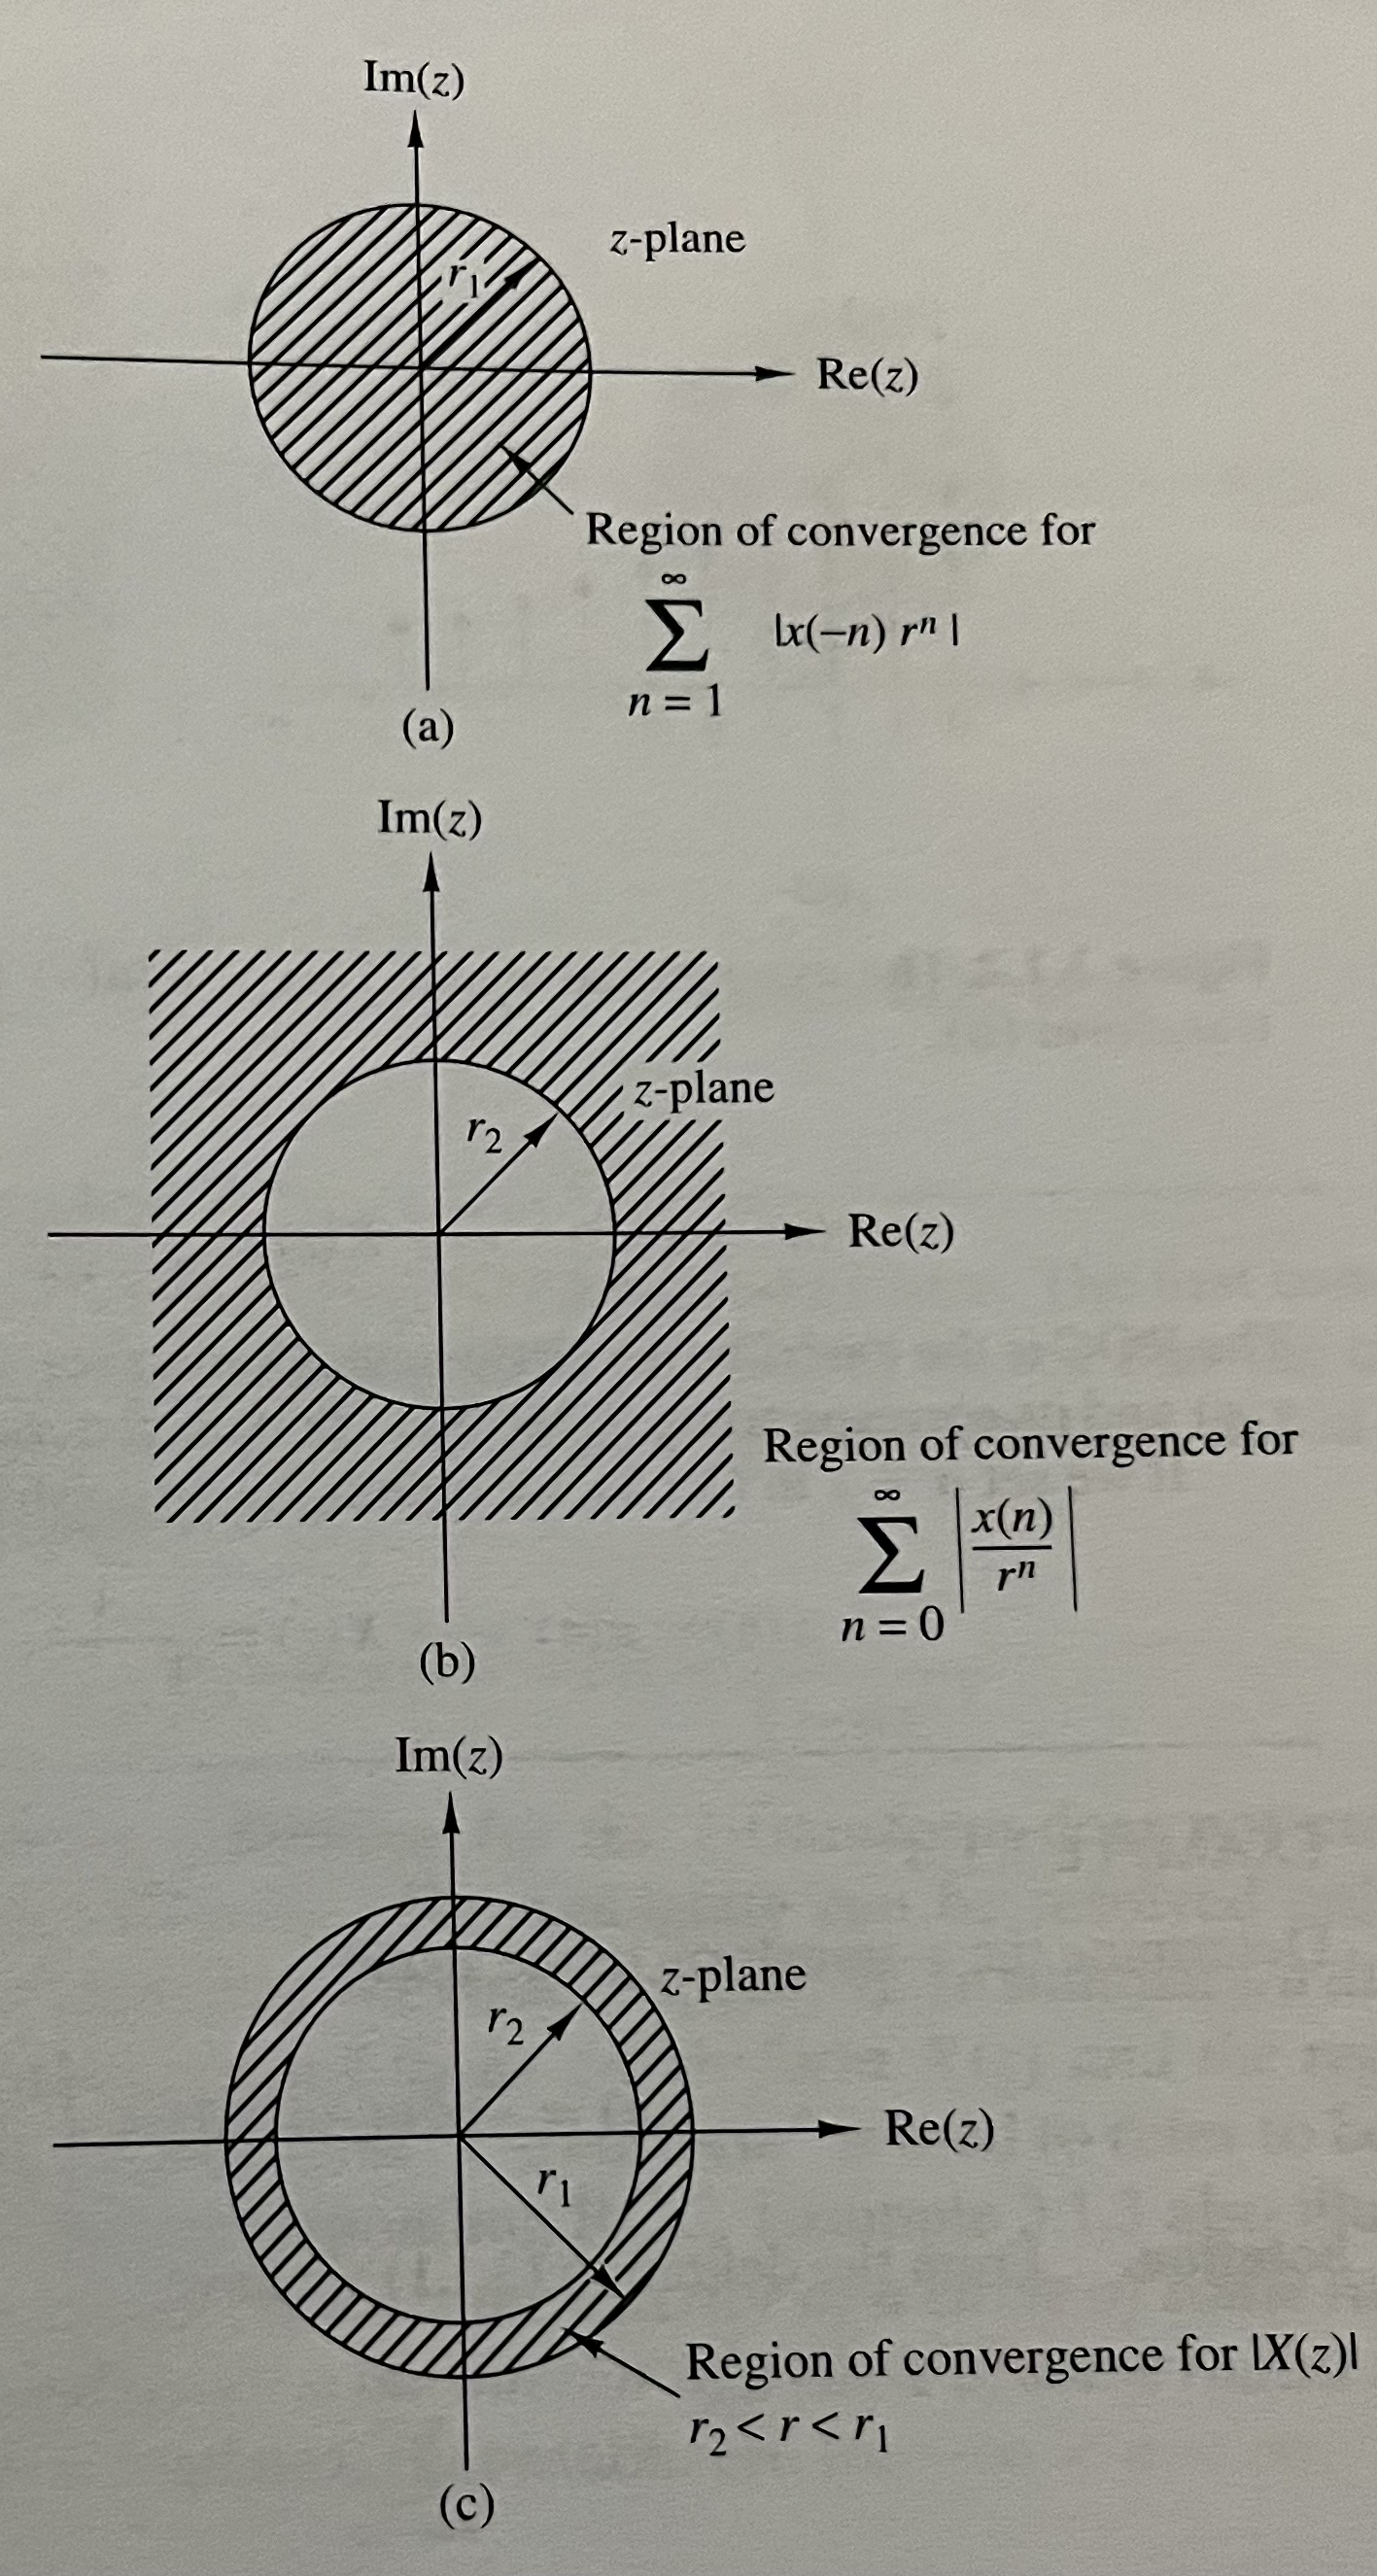
\includegraphics[width=5cm]{roc}
	\caption{ROC Example}
	\end{figure}
	
	The z-transform without an ROC doesnt uniquely specify the signal in the time domain. For example
	\begin{equation}
	Z{\alpha^nu[n]}  = Z{-\alpha^nu[-n-1]} = \frac{1}{1-\alpha z^{-1}}
	\end{equation}
	This shows you would need the ROC to tell the difference of the z-transforms without the ROC. The ROC of a causal signal is the exterior of a circle of some radius $r_2$ while the ROC of a non-causal signal is the interior of the circle. If a signal is infinite and two sided then the ROC is a ring in the z-plane. The figure 2 shows characteristic families of signals and their ROC's.
	
	\begin{figure}[h]
	\centering
	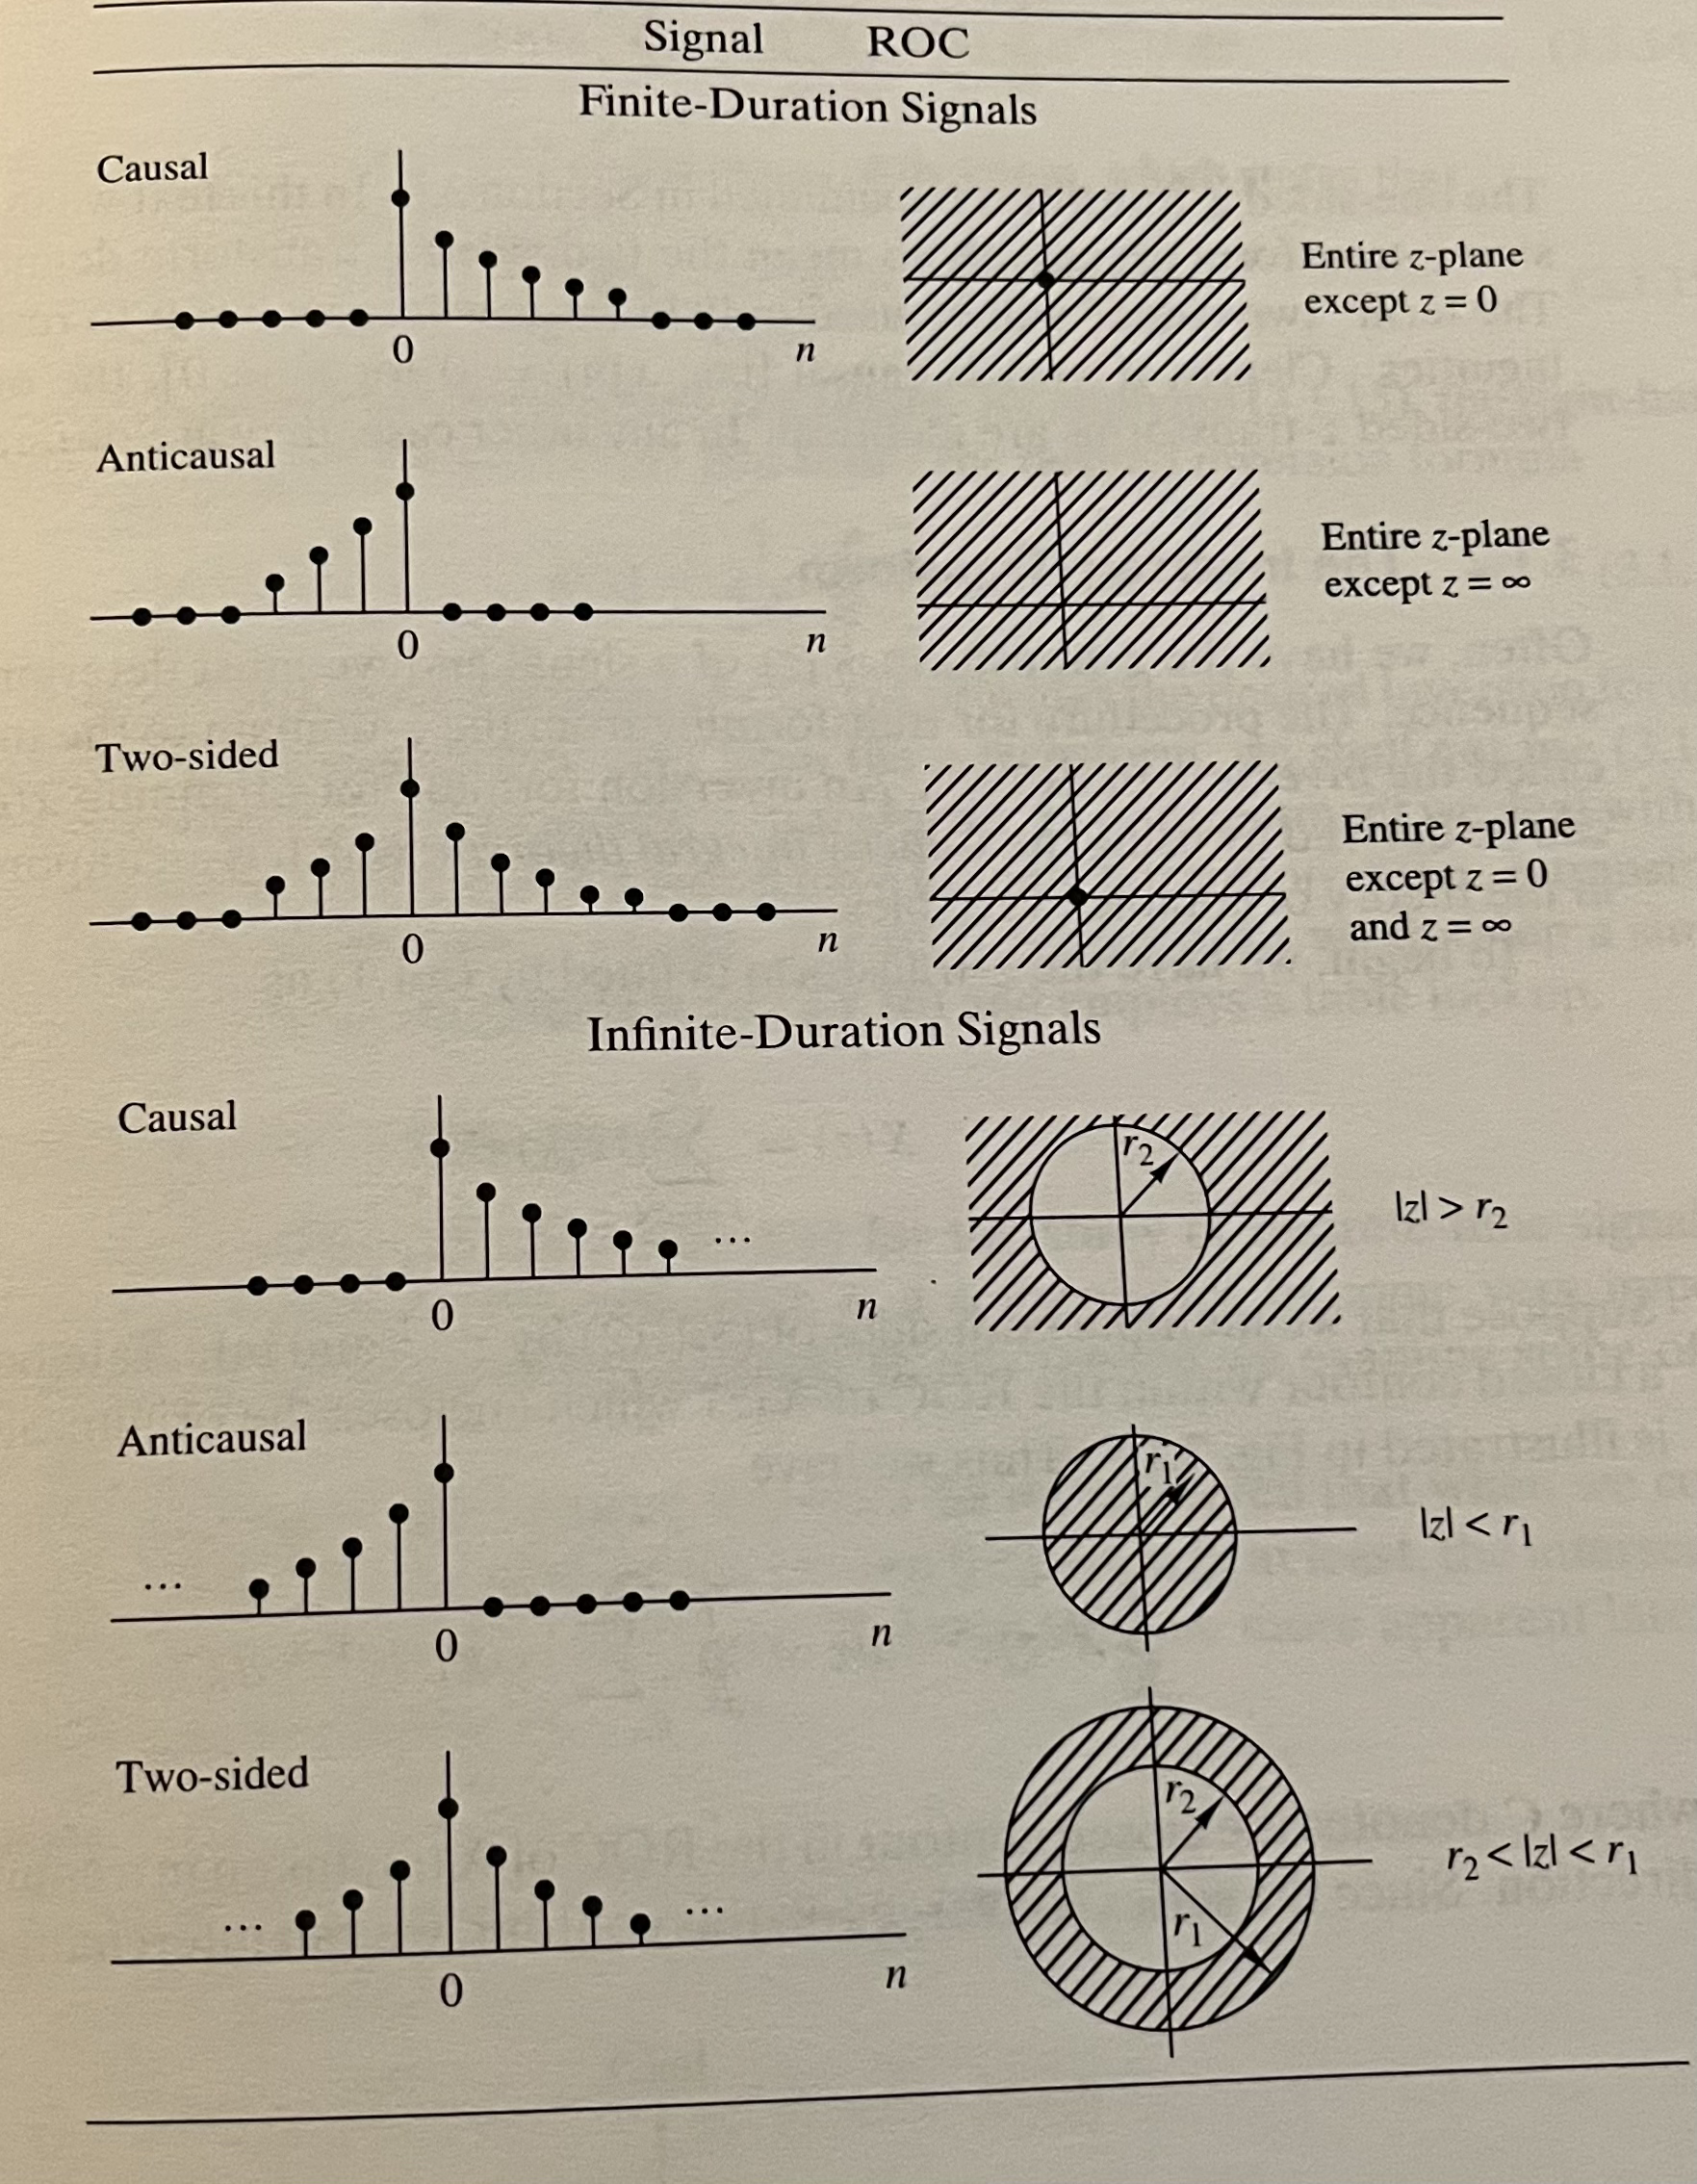
\includegraphics[width=5cm]{fam}
	\caption{Characteristic Families of Signals and their corresponding ROC's}
	\end{figure}
	
	The z-transform defined in eqn 1 if referred to as the \textit{two-sided} or \textit{bilateral} z-transform to distinguish it from the \textit{one-sided} or \textit{unilateral} z-transform given by
	\begin{equation}
	X^+(z) = \sum_{n=0}^{\infty}x[n]z^{-n}
	\end{equation}
	
	\subsection{The Inverse z-Transform}
	The inverse z-transform is defined as 
	\begin{equation}
	x[n] = \frac{1}{2\pi j} \oint_C X(z)z^{n-1}dz
	\end{equation}
	where the integral is the contour integral over a contour that encloses the origin. This is complicated and later this chapter an easier inverse z-transform is shown.
	
	\section{Properties of the z-Transform}
	The important properties of the z-Transform are shown in the figure 3.
	
	\begin{figure}[h]
	\centering
	\includegraphics[width=6cm]{zprop}
	\caption{Properties of z-Tranform}
	\end{figure}
	
	And common z-Transform pairs are shown on page 170.
	
	\section{Rational z-Transform}
	An important family of z-transforms are those where $X(z)$ is a rational function.
	\subsection{Poles and Zeros}
	The \textit{zeros} of $X(z)$ are the values of z for which $X(z) = 0$ and the poles are when $X(z) = \infty$. 
	\begin{equation}
	X(z) = \frac{B(z)}{A(z)} = \frac{b_0 + b_1z^{-1}+ ... + b_Mz^{-M}}{a_0 + a_1z^{-1}+ ... + a_Nz^{-N}} = \frac{\sum_{k=0}^M b_kz^{-k}}{\sum_{k=0}^N a_kz^{-k}}
	\end{equation}
	If $a_0 != 0$ and $b_0 != 0$ then we can avoid the negative powers of $z$ we can factor out
	\begin{equation}
	\frac{b_0z^{-M}}{a_0z^{-N}}
	\end{equation}
	and since $B(z)$ and $A(z)$ are polynomials we can express $X(z)$ as
	\begin{equation}
	X(z) = Gz^{N-M} \frac{\Pi_{k=1}^M (z-z_k)}{\Pi_{k=1}^N(z-p_k)}
	\end{equation}
	where $G = b_0/a_0$ where the zeros are $z_k$ and poles $p_k$. You can represent $X(z)$ as a \textit{pole-zero} plot where the poles are represented as crosses (x) and the zeros are represented with circles $\circ$. The $|X(z)|$ is a 2-D function that describes a surface. 
	\subsection{Pole Location and TD Behavior for Causal Signals}
	This subsection covers the relationship between the zeros and poles and the corresponding Real, Causal time domain signal. The next 3 figures show the poles/zeros and the corresponding time domain signal. 
	
	\begin{figure}[h]
	\centering
	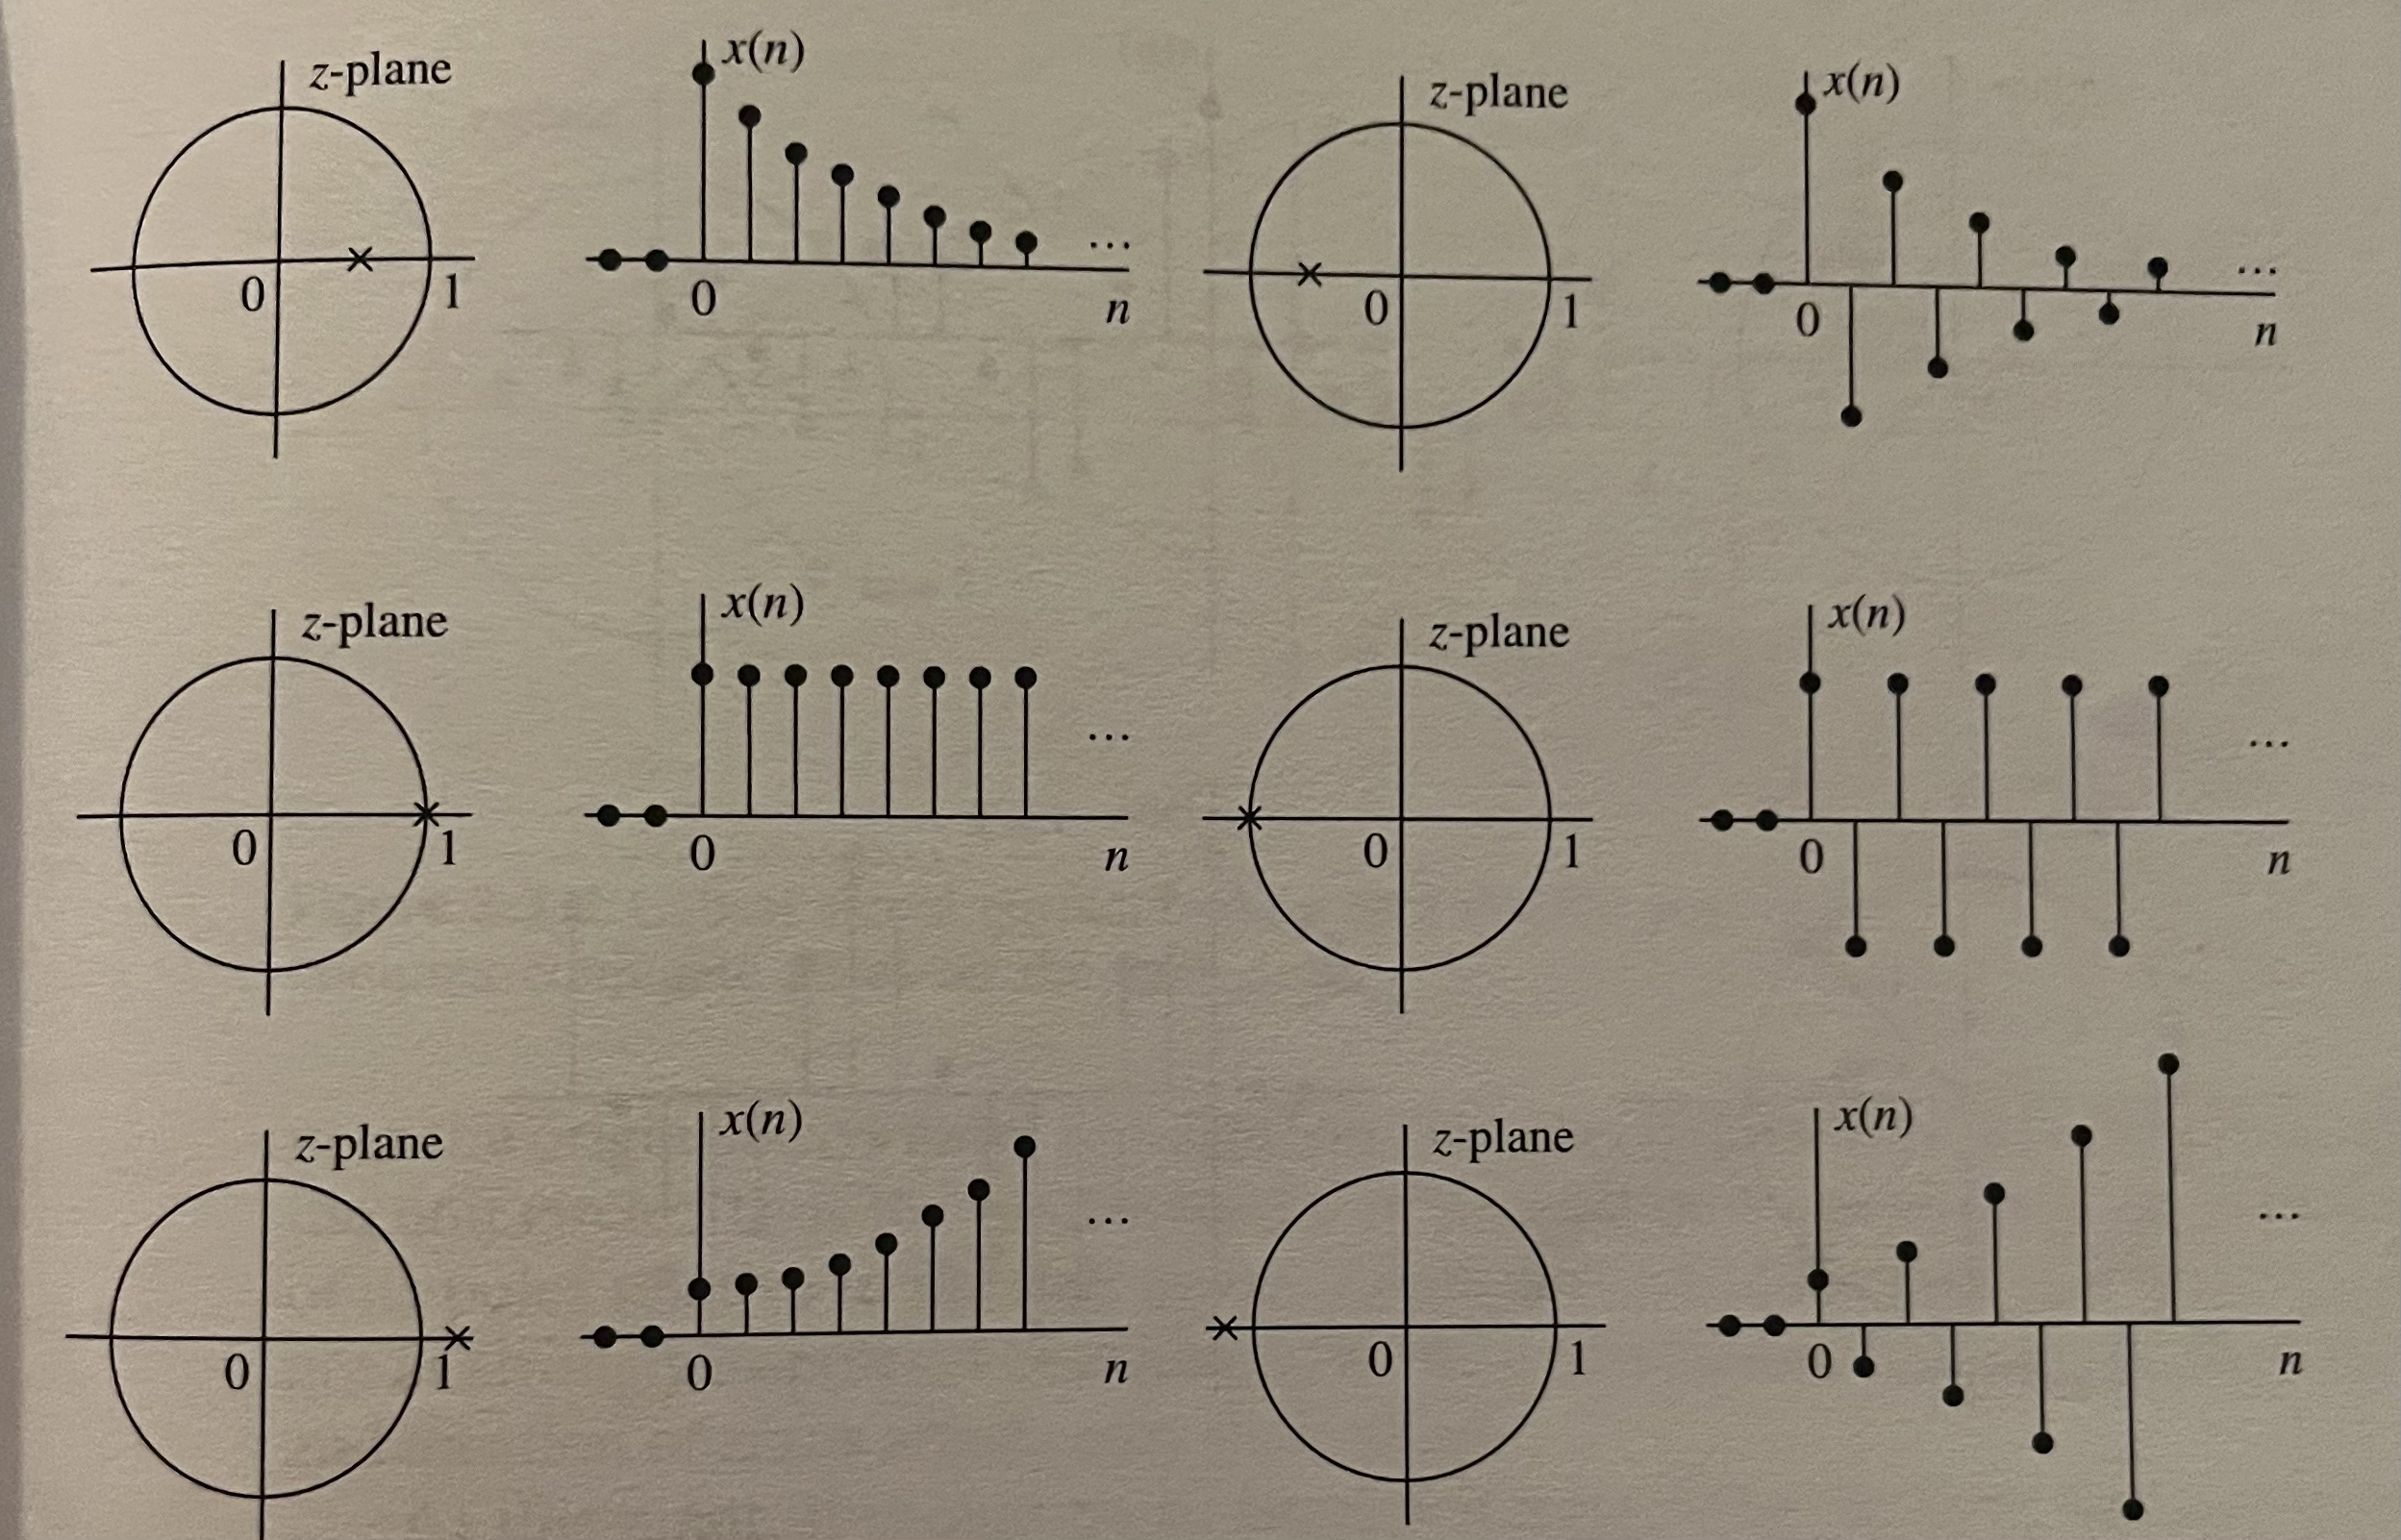
\includegraphics[width=5cm]{srp}
	\caption{Single real pole causal signal}
	\end{figure}
	
	\begin{figure}[h]
	\centering
	\includegraphics[width=5cm]{drp}
	\caption{Double real pole of causal signals}
	\end{figure}
	
	\begin{figure}[h]
	\centering
	\includegraphics[width=5cm]{ccp}
	\caption{Complex Conjugate poles}
	\end{figure}
	
	\subsection{The System Function of a LTI Signal}
	\begin{equation}
	Y(z) = H(z)X(z)
	\end{equation}
	\begin{equation}
	\frac{Y(z)}{X(z)} = H(z) = \frac{\sum_{k=0}^Mb_kz^{-k}}{1 + \sum_{k=1}a_kz^{-k}}
	\end{equation}
	A LTI system can be described by a constant-coefficient difference equation that has a rational system function. There are two other important system functions. One for when $a_k = 0$ for $1 \le k \le N$,
	\begin{equation}
	H(z) = \sum_{k=0}^Mb_kz^{-k} = \frac{1}{z^M} \sum_{k=0}^Mb_kz^{M-k}
	\end{equation}
	and for when $b_k = 0$ for $1 \le k \le M$, 
	\begin{equation}
	H(z) = \frac{b_0}{1+\sum_{k=1}^Na_kz^{-k}} = \frac{b_0z^N}{\sum_{k=0}^Na_kz{N-k}}
	\end{equation}
	
	\section{Inversion of the z-Transform}
	The contour integral shown earlier over a closed path $C$ can give $x[n]$. The three methods to get $x[n]$ from $X(z)$ are\\
	\textbf{1.} Direct evaluation with contour integrals.\\
	\textbf{2.} Expansion into a series of terms with the variables $z$ and $z^{-1}$\\
	\textbf{3.} Partial-fraction expansion and table lookup
	
	\subsection{The Inverse z-Transform with Contour Integration}
	When the proper fraction $f(z)/g(z)$, where $f(z)$ has no poles inside the contour $C$ and $g(z)$ is a polynomial with distinct simple roots then
	\begin{equation}
	\frac{1}{2\pi j} \oint_c \frac{f(z)}{g(z)}dz = \sum_{i=1}^n A_i
	\end{equation}
	where
	\begin{equation}
	A_i = (z-z_i)\frac{f(z)}{g(z)}|_{z=z_i}
	\end{equation}
	In the case of the inverse z-transform
	\begin{equation}
	x[n] = \sum_i (z-z_i)X(z)z^{n-1}|_{z=z_i}
	\end{equation}
	provided the poles are simple.
	
	\subsection{The inverse z-Transform by Power Series Expansion}
	Given a z-transform $X(z)$ with the corresponding ROC we can expand it into the power series form
	\begin{equation}
	X(z) = \sum_n c_nz^{-n}
	\end{equation}
	which converges in the given ROC. Then by the uniqueess of the z-transform $x[n] = c_n$ for all $n$. In general the method of long division shown in example 3.4.2b will not provide answers for $x[n]$ when $n$ is large since the long division becomes tedious. It is used to find the values of the first few samples of the signal.
	
	\subsection{The Inverse z-Transform by Partial-Fraction Expansion}
	In the table lookup method we attempt to express $X(z)$ as a linear combination
	\begin{equation}
	X(z) = \alpha_1X_1(z) + \alpha_2X_2(z) + ... \alpha_kX_k(z)
	\end{equation}
	where the $X_k$ values are the transforms are $x_k$ available in the transform table. Without loss of generality we assume $a_0 = 1$ so 
	\begin{equation}
	X(z) = \frac{B(z)}{A(z)} = \frac{b_0 + b_1z^{-1} + ... + b_Mz^{-M}}{1 + a_1z^{-1} + ... + a_Nz^{-N}}
	\end{equation}
	If $a_0 != 1$ then divide by $a_0$. A rational function of the form in the preceeding equation is \textit{proper} if $a_N != 0$ and $M < N$. The number of zeros is less than poles. An improper rational function can be written as the sum of a polynomial and a proper rational function. This section covers the partial fraction expansion of proper polynomials since improper ones can be manipulated into proper form. Let
	\begin{equation}
	X(z) = \frac{B(z)}{A(z)} = \frac{b_0 + b_1z^{-1} + ... + b_Mz^{-M}}{1 + a_1z^{-1} + ... + a_Nz^{-N}}
	\end{equation}
	where 
	\begin{equation}
	x_n != 0 \text{ and } M < N
	\end{equation}
	You can multiply both sides by $z^N$. The function of partial-fraction expansion is to express the prior equation as a sum of simple fractions. We first factor the denominator polynomial nto factors that contain the poles $p_1, p_2 ... p_N$. There are two main cases\\
	\textbf{Distinct Poles}\\
	Suppose that the poles are all different (distinct) where
	\begin{equation}
	\frac{X(z)}{z} = \frac{A_1}{z-p_1} + \frac{A_2}{z-p_2} + ... + \frac{A_N}{z-p_N}
	\end{equation}
	and the problem is to determine the coefficients $A_1, A_2, ..., A_N$. We can determine the coefficients by multiplying both sides by each of the terms $(z-p_k)$ and evaluating the resulting expressions at the corresponding pole positions. Example on page 186. This holds for both real and complex poles. Complex conjugate poles result in complex-conjugate coefficients in the partial fraction expansion. \\
	\textbf{Multiple-order Poles}\\
	If $X(z)$ has a pole of multiplicity $l$ that is $(z-p_k)^l$ then the previous method no longer holds. The partial fraction expanstion must contain the terms 
	\begin{equation}
	\frac{A_{1k}}{z-p_k} + \frac{A_{2k}}{(z-p_k)^2} + ... + \frac{A_{mk}}{(z-p_k)^m}
	\end{equation}	 
	You can now solve this the same way that you would with distinct poles. To find the inverse z-transform of the partial fraction expantion, you can find the z-transform by inverting each of the individual terms. 
	
	\section{Analysis of LTI Systems in the z-Domain}
	\subsection{Response of Systems with Rational System Functions}
	Assume that $H(z) = B(z)/A(z)$ and $X(z) = N(z)/Q(z)$, and is relaxed (initial conditions are zero) then
	\begin{equation}
	Y(z) = H(z)X(z) = \frac{B(z)N(z)}{A(z)Q(z)}
	\end{equation}
	Assume the poles of the system equation $p_k$ dont equal the poles of the signal $q_m$ for all $k$ and $m$ and there are no pole-zero cancellations. 
	\begin{equation}
	y[n] = \sum_{k=1}^N A_k(p_k)^nu[n] + \sum_{k=1}^L Q_k(q_k)^n u[n]
	\end{equation}
	The \textit{natural response} of the system is the first sum with the poles of the system and the \textit{forced response} of the system is the second sum with the poles of the signal.$A_k$ and $Q_k$ are functions of both sets of poles. If $X(z)$ and $H(z)$ have one or more poles in common and or when they contain multiple order poles, $Y(z)$ will have multiple order poles.
	
	\subsection{transient and Steady State Response}
	The natural response of a causal system is 
	\begin{equation}
	y_{nr}[n] = \sum_{k=1}^NA_k(p_k)^nu[n]
	\end{equation}
	If $|p_k| < 1$ for all k then the \textit{natural response} will decay to zero and is called the \textit{transient response}.
	
	The forced response is 
	\begin{equation}
	y_{fr}[n] = \sum_{k=1}^L Q_k(q_k)^Nu[n]
	\end{equation}
	If all the poles of the input signal fall inside the unit circle it will decay to zero. If the poles of the input circle fall on the unit circle (sinusoid) then this is called the \textit{steady state response}.
	\subsection{Causality and Stability}
	A LTI system if causal if and only if the ROC of the system function if the exterior of a circle approaching $\infty$ and includes $\infty$. In order to be stable, the ROC must include the unit circle.

	\subsection{Pole-Zero Cancellations}
	By having a pole-zero cancellation in $X(z)$ and $H(z)$ you can suppress different aspects of a signal.
	
	\subsection{Multiple-Order Poles and Stability}
	In order for a system to be BIBO stable all poles must be inside the unit circle.
	
	\subsection{Stability of Second Order Systems}
	\begin{equation}
	H(z) = \frac{b_0z^2}{z^2+a_1z+a2}
	\end{equation}
	A two-pole system is stable if and only if the coefficients satisfy
	\begin{equation}
	|a_2| = |p_1p_2| = |p_1||p_2| < 1
	\end{equation}
	\begin{equation}
	|a_1| < 1 + a_2
	\end{equation}\\
	\textbf{Real and Distinct Poles}\\
	Since $p_1$, $p_2$ are real and $p_1 != p_2$
	\begin{equation}
	h[n] = \frac{b_0}{p_1-p_2}(p_1^{n+1}-p_2^{n+1})u[n]
	\end{equation}
	\textbf{Real and equal Poles}\\
	In this case $p_1 = p_2 = -a_1/2$
	\begin{equation}
	H(z) = \frac{b_0}{(1-pz^{-1})^2}
	\end{equation}
	\begin{equation}
	h[n] = b_0(n+1)p^nu[n]
	\end{equation}
	\textbf{Complex Conjugate poles}\\
	Since the poles are complex conjugate,
	\begin{equation}
	H(z) = \frac{A}{1-re^{j\omega_0}z^{-1}} + \frac{A^*}{1-re^{-j\omega_0}z^{-1}}
	\end{equation}
	\begin{equation}
	A = \frac{b_0 e^{j\omega_0}}{j2\sin \omega_0}
	\end{equation}
	\begin{equation}
	h[n] = \frac{b_0 r^n}{\sin(n+1)\omega_0u[n]}
	\end{equation}
	
	 \section{One-Sided z-Transform}
	In this section, one-sided z-Transforms are developed to sole difference equations with initial conditions. 
	\subsection{Definition and Properties}
	The \textit{one sided} or \textit{unilateral} z-transform of a signal $x[n]$ is 
	\begin{equation}
	X^+(z) = \sum_{n=0}^{\infty} x[n]z^{-n}
	\end{equation}
	This differs from the two sided transform in the following ways,\\
	\textbf{1.} It doesn't contain information about the signal $x[n]$ for $n < 0$\\
	\textbf{2.} It is \textit{unique} only for causal signals\\
	\textbf{3.} The unilateral z-transform is identical to the bilateral z-transform of the signal $x[n]u[n]$\\
	
	Almost all the properties of the z-transform carry over except for the time-shifting property. 
	\textbf{Case 1. Time Delay}
	\begin{equation}
	x[n-k] \leftrightarrow^{z^+} z^{-k}[X^+(z) + \sum_{n=1}^kx[-n]z^n
	\end{equation}
	And if $x[n]$ is causal then
	\begin{equation}
	x[n-k] \leftrightarrow^{z^+} z^{-k}X^+(z)
	\end{equation}
	\textbf{Time Advance}
	\begin{equation}
	x[n+k] \leftrightarrow^{z^+} z^k[X^+(z) - \sum_{n=0}^{k-1}x[n]z^{-n}
	\end{equation}
	
	An important theorem useful in the analysis of signals and systems is the \textbf{final value theorem:}
	\begin{equation}
	\lim_{n \rightarrow \infty} x[n] = \lim_{z \rightarrow 1} (z-1)X^+(z)
	\end{equation}
	And this exists if the ROC of the right hand side includes the unit circle.
	
	\subsection{Solution of Difference Equations}
	Examples on page 210
	
	\subsection{Response of Pole-Zero systems with Nonzero Initial Conditions}
	\begin{equation}
	Y^+(z) = X(z)H(z) + \frac{N_0(z)}{A(z)}
	\end{equation}
	where 
	\begin{equation}
	N_0(z) = -\sum_{k=1}^N a_kz^{-k} \sum_{n=1}^k y(-n)z^n
	\end{equation}	
	
\end{document} % This is the end of the document